\documentclass[11pt]{article}
\usepackage{icmlko}
\begin{document}

\title{집안 손님도 손님이다 --- 도메인 하나씩 빼서 전이 시험대를 열한 개로}
\author{월드모델 실험실}
\date{노트 430 · 2026년 8월 4일}
\maketitle

\begin{abstract}
노트 429가 안 본 도메인 짝 둘이 처음으로 갈리는 것을 보고 ``셋째 짝이
급하다''로 닫았다. 새 도메인을 모으는 대신 \textbf{있는 도메인을 하나씩
학습에서 빼서} 전이 시험대로 썼다 --- 도메인 $d$ 의 2025년 이전 행을 한 줄도
안 넣고 나머지 열로 학습해 $d$ 의 유보 행을 채점한다. $d$ 는 원핫이 전부 0 인
좌표를 받는다. \textbf{짝이 둘에서 열하나가 된다.}

기구 검사를 사전 등록했다 --- \emph{LODO 도메인은 같은 수집 · 같은 라벨
계기를 쓰니 KR 만화($+0.2314$)보다 다 높을 것이다.}

\begin{center}
\begin{tabular}{lrrr}
\hline
뺀 도메인 & LODO 전이 & 판에 있을 때 & 차 \\
\hline
게임 & $+0.5262$ & $+0.6535$ & $0.13$ \\
세계애니 & $+0.3958$ & $+0.5627$ & $0.17$ \\
도서 & $+0.3607$ & $+0.3750$ & $0.01$ \\
팝업 & $+0.3447$ & $+0.3944$ & $0.05$ \\
애니 & $+0.2567$ & $+0.5369$ & $0.28$ \\
만화 & $+0.2312$ & $+0.3544$ & $0.12$ \\
모바일 & $+0.2130$ & $+0.6195$ & $0.41$ \\
시장팝업 & $+0.1343$ & $+0.1368$ & $\mathbf{0.00}$ \\
웹툰 & $+0.0423$ & $+0.4612$ & $\mathbf{0.42}$ \\
아이돌 & $+0.0357$ & $+0.4313$ & $0.40$ \\
\textbf{펀딩} & $\mathbf{-0.0233}$ & $+0.3706$ & $0.39$ \\
\hline
\end{tabular}
\end{center}

\textbf{반증됐다.} 열하나 중 \textbf{여섯이 KR 만화보다 낮고} 펀딩은
\textbf{음수}다. \textbf{같은 수집에서 왔다고 친한 손님이 아니다.}
\end{abstract}

\section{KR 만화는 평범한 손님이었다}

LODO 열하나의 평균이 $+0.2288$ 이고 KR 만화가 $+0.2314$ 다. \textbf{거의
같다.} 이 사이클 내내 결론을 지고 온 그 짝이 \textbf{유난히 어려운 손님도
쉬운 손님도 아니었다} --- 뒤늦게나마 그 선택이 치우치지 않았다는 증거가
생겼다. (비게임 앱 $+0.1730$ 은 조금 아래다.)

\section{학습에 드는 것의 값}

새 눈금이 하나 생겼다 --- \textbf{판에 있을 때 $-$ 빼고 나면}. 이것이 그
도메인이 ``학습에 든다''는 사실에서 얻는 값이다.

\begin{center}
시장팝업 $0.00$ · 도서 $0.01$ · 팝업 $0.05$ $\ \cdots\ $
모바일 $0.41$ · 웹툰 $0.42$
\end{center}

\textbf{$0.00$ 에서 $0.42$ 까지 벌어진다.} 시장팝업은 학습에 있으나 없으나
같은 점수를 받는다 --- 제 이력에서 배우는 것이 없고 남의 축만 빌려 쓴다는
뜻이다(노트 425가 그 도메인 축을 못 실은 것과 같은 그림). 반대로 웹툰과
모바일은 자기 이력이 성적의 대부분이다.

이 눈금은 판이 못 보던 것이다. 판에서 웹툰 $+0.4612$ 와 세계애니 $+0.5627$ 은
비슷해 보이는데, 빼 보면 $+0.0423$ 과 $+0.3958$ 로 갈린다.

\section{판을 잘하는 것과 안 본 채로 맞히는 것은 다르다}

LODO 와 판의 순위상관이 $+0.445$ 다. \textbf{판에서 잘하는 도메인이 안 본
채로도 잘 맞는다는 보장이 없다} --- 게임은 둘 다 1등이지만 모바일은 판 2등에
LODO 7등이다.

이것은 노트 423·425가 \emph{변경}에 대해 말한 것(판이 목표를 못 본다)을
\emph{도메인}에 대해 다시 말한다.

\section{남은 것}

\begin{tabular}{lp{7.0cm}}
\hline
$K{=}64$ 를 열한 짝으로 & 이 시험대를 지은 원래 이유다(노트 429가 못 정했다) \\
규약을 다수결로 & ``둘 이상 같은 부호''를 ``열하나 중 몇'' 으로 올릴 수 있다 \\
펀딩이 음수 & 학습에 없으면 거꾸로 줄을 세운다. KR 만화가 그랬던 자리
(노트 398)이고, 그때는 원핫이 범인이었다 \\
씨앗 셋 & 절대값의 잡음을 안 쟀다. 견줄 때는 짝지으므로 덜 문제다 \\
\hline
\end{tabular}

\begin{figure}[h]
\centering
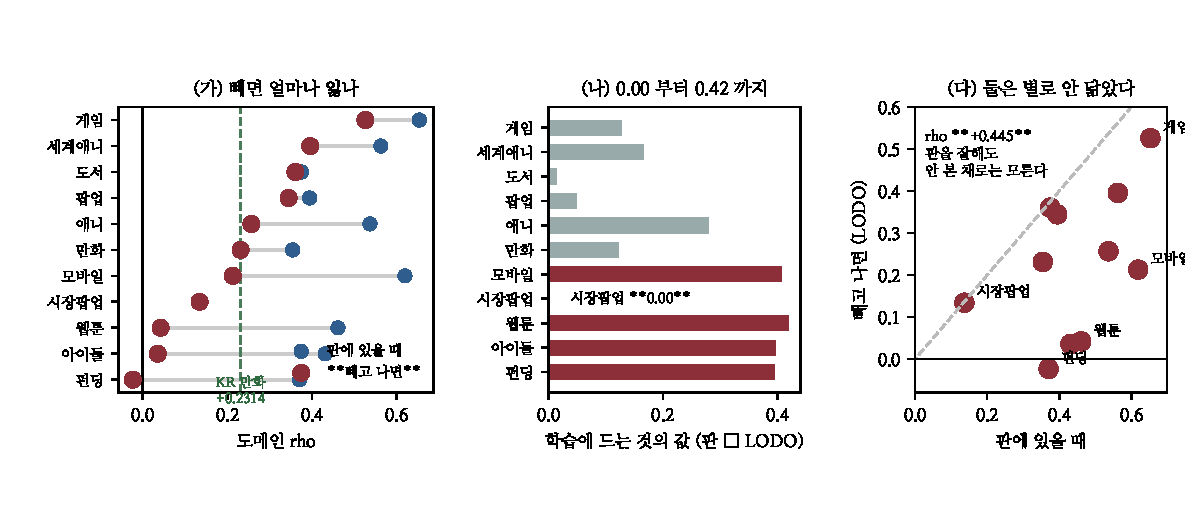
\includegraphics[width=\textwidth]{figs/fig430.pdf}
\caption{(가) 도메인마다 빼면 얼마나 잃나. 초록 선이 KR 만화. (나) 학습에
드는 것의 값이 $0.00$ 에서 $0.42$ 까지. (다) 판과 LODO 는 $\rho = +0.445$
로만 닮았다.}
\end{figure}

\end{document}
